%%========================================================================
%% LaTeX sjabloon voor stage/projectrapport of bachelorproef
%%  HoGent Bedrijf en Organisatie
%%========================================================================

%%========================================================================
%% Preamble
%%========================================================================

\documentclass[pdftex,a4paper,12pt,twoside]{report}

% XXX: Let op: dit sjabloon is gemaakt om dubbelzijdig af te drukken
% Voor enkelzijdig, verwijder ``twoside'' hierboven.

%%---------- Extra functionaliteit ---------------------------------------

\usepackage[utf8]{inputenc}  % Accenten gebruiken in tekst (vb. é ipv \'e)
\usepackage{amsfonts}        % AMS math packages: extra wiskundige
\usepackage{amsmath}         %   symbolen (o.a. getallen-
\usepackage{amssymb}         %   verzamelingen N, R, Z, Q, etc.)
%\usepackage[dutch]{babel}   % Taalinstellingen: woordsplitsingen,
                             %  commando's voor speciale karakters
                             %  ("dutch" voor NL)
\usepackage{eurosym}         % Euro-symbool €
\usepackage{geometry}
\usepackage{graphicx}        % Invoegen van tekeningen
\usepackage[pdftex,bookmarks=true]{hyperref}
                             % PDF krijgt klikbare links & verwijzingen,
                             %  inhoudstafel
\usepackage{epigraph}
\usepackage{listings}        % Broncode mooi opmaken
\usepackage{multirow}        % Tekst over verschillende cellen in tabellen
\usepackage{rotating}        % Tabellen en figuren roteren
\usepackage{natbib}          % Betere bibliografiestijlen
\usepackage{fancyhdr}        % Pagina-opmaak met hoofd- en voettekst

\usepackage[T1]{fontenc}     % Ivm lettertypes
\usepackage{lmodern}
\usepackage{textcomp}

%%---------- Layout ------------------------------------------------------

% hoofdingen, enz.
\pagestyle{fancy}
% enkel hoofdstuktitel in hoofding, geen sectietitel (vermijd overlap)
\renewcommand{\sectionmark}[1]{}

% lijn, wordt gebruikt in titelpagina
\newcommand{\HRule}{\rule{\linewidth}{0.5mm}}

% Leeg blad
\newcommand{\emptypage}{
\newpage
\thispagestyle{empty}
\mbox{}
\newpage
}

% Gebruik een schreefloos lettertype ipv het "oubollig" uitziende
% Computer Modern
\renewcommand{\familydefault}{\sfdefault}

% Commando voor invoegen Java-broncodebestanden (dank aan Niels Corneille)
% Gebruik: \codefragment{source/MijnKlasse.java}{Uitleg bij de code}
\newcommand{\codefragment}[2]{ \lstset{%
  language=java,
  breaklines=true,
  float=th,
  caption={#2},
  basicstyle=\scriptsize,
  frame=single,
  extendedchars=\true
}
\lstinputlisting{#1}}

%%---------- Documenteigenschappen ---------------------------------------
%% Vul dit aan met je eigen info:

% Je eigen naam
\newcommand{\student}{Jan {Van Braeckel}}

% De naam van je lector, begeleider, promotor
\newcommand{\promotor}{Joeri {Van Herreweghe}}

% De naam van je co-promotor
\newcommand{\copromotor}{Peter Leemans}

% Indien je bachelorproef in opdracht van een bedrijf of organisatie
% geschreven is, geef je hier de naam.
\newcommand{\instelling}{AllThingsTalk}

% De titel van het rapport/bachelorproef
\newcommand{\titel}{Bluetooth Low Energy wearables in een Internet of Things cloud-infrastructuur met behulp van een smartphone als gateway}
\newcommand{\titleEN}{Bluetooth Low Energy wearables in an Internet of Things cloud infrastructure using a smartphone as gateway}

% Datum van indienen
\newcommand{\datum}{27 mei 2015}

% Faculteit
\newcommand{\faculteit}{Faculteit `Bedrijf en Organisatie'}
\newcommand{\faculty}{Faculty `Bedrijf en Organisatie'}

% Soort rapport
\newcommand{\rapporttype}{Scriptie voorgedragen tot het bekomen van de graad\\Bachelor in de toegepaste informatica}
\newcommand{\reporttype}{Thesis submitted in fulfillment of the requirements for the degree of\\Bachelor in applied computer sciences}

% Academiejaar
\newcommand{\academiejaar}{2015-2016}

% Examenperiode
%  - 1e semester = 1e examenperiode
%  - 2e semester = 2e examenperiode
%  - tweede zit = 3e examenperiode
\newcommand{\examenperiode}{Tweede examenperiode}
\newcommand{\examperiod}{Second exam period}

%%========================================================================
%% Inhoud document
%%========================================================================

\begin{document}

%%---------- Front matter ------------------------------------------------
%% Het voorblad - Hier moet je in principe niets wijzigen.

\begin{titlepage}
  \newgeometry{top=2cm,bottom=1.5cm,left=1.5cm,right=1.5cm}
  \begin{center}

    \begingroup
    \rmfamily
    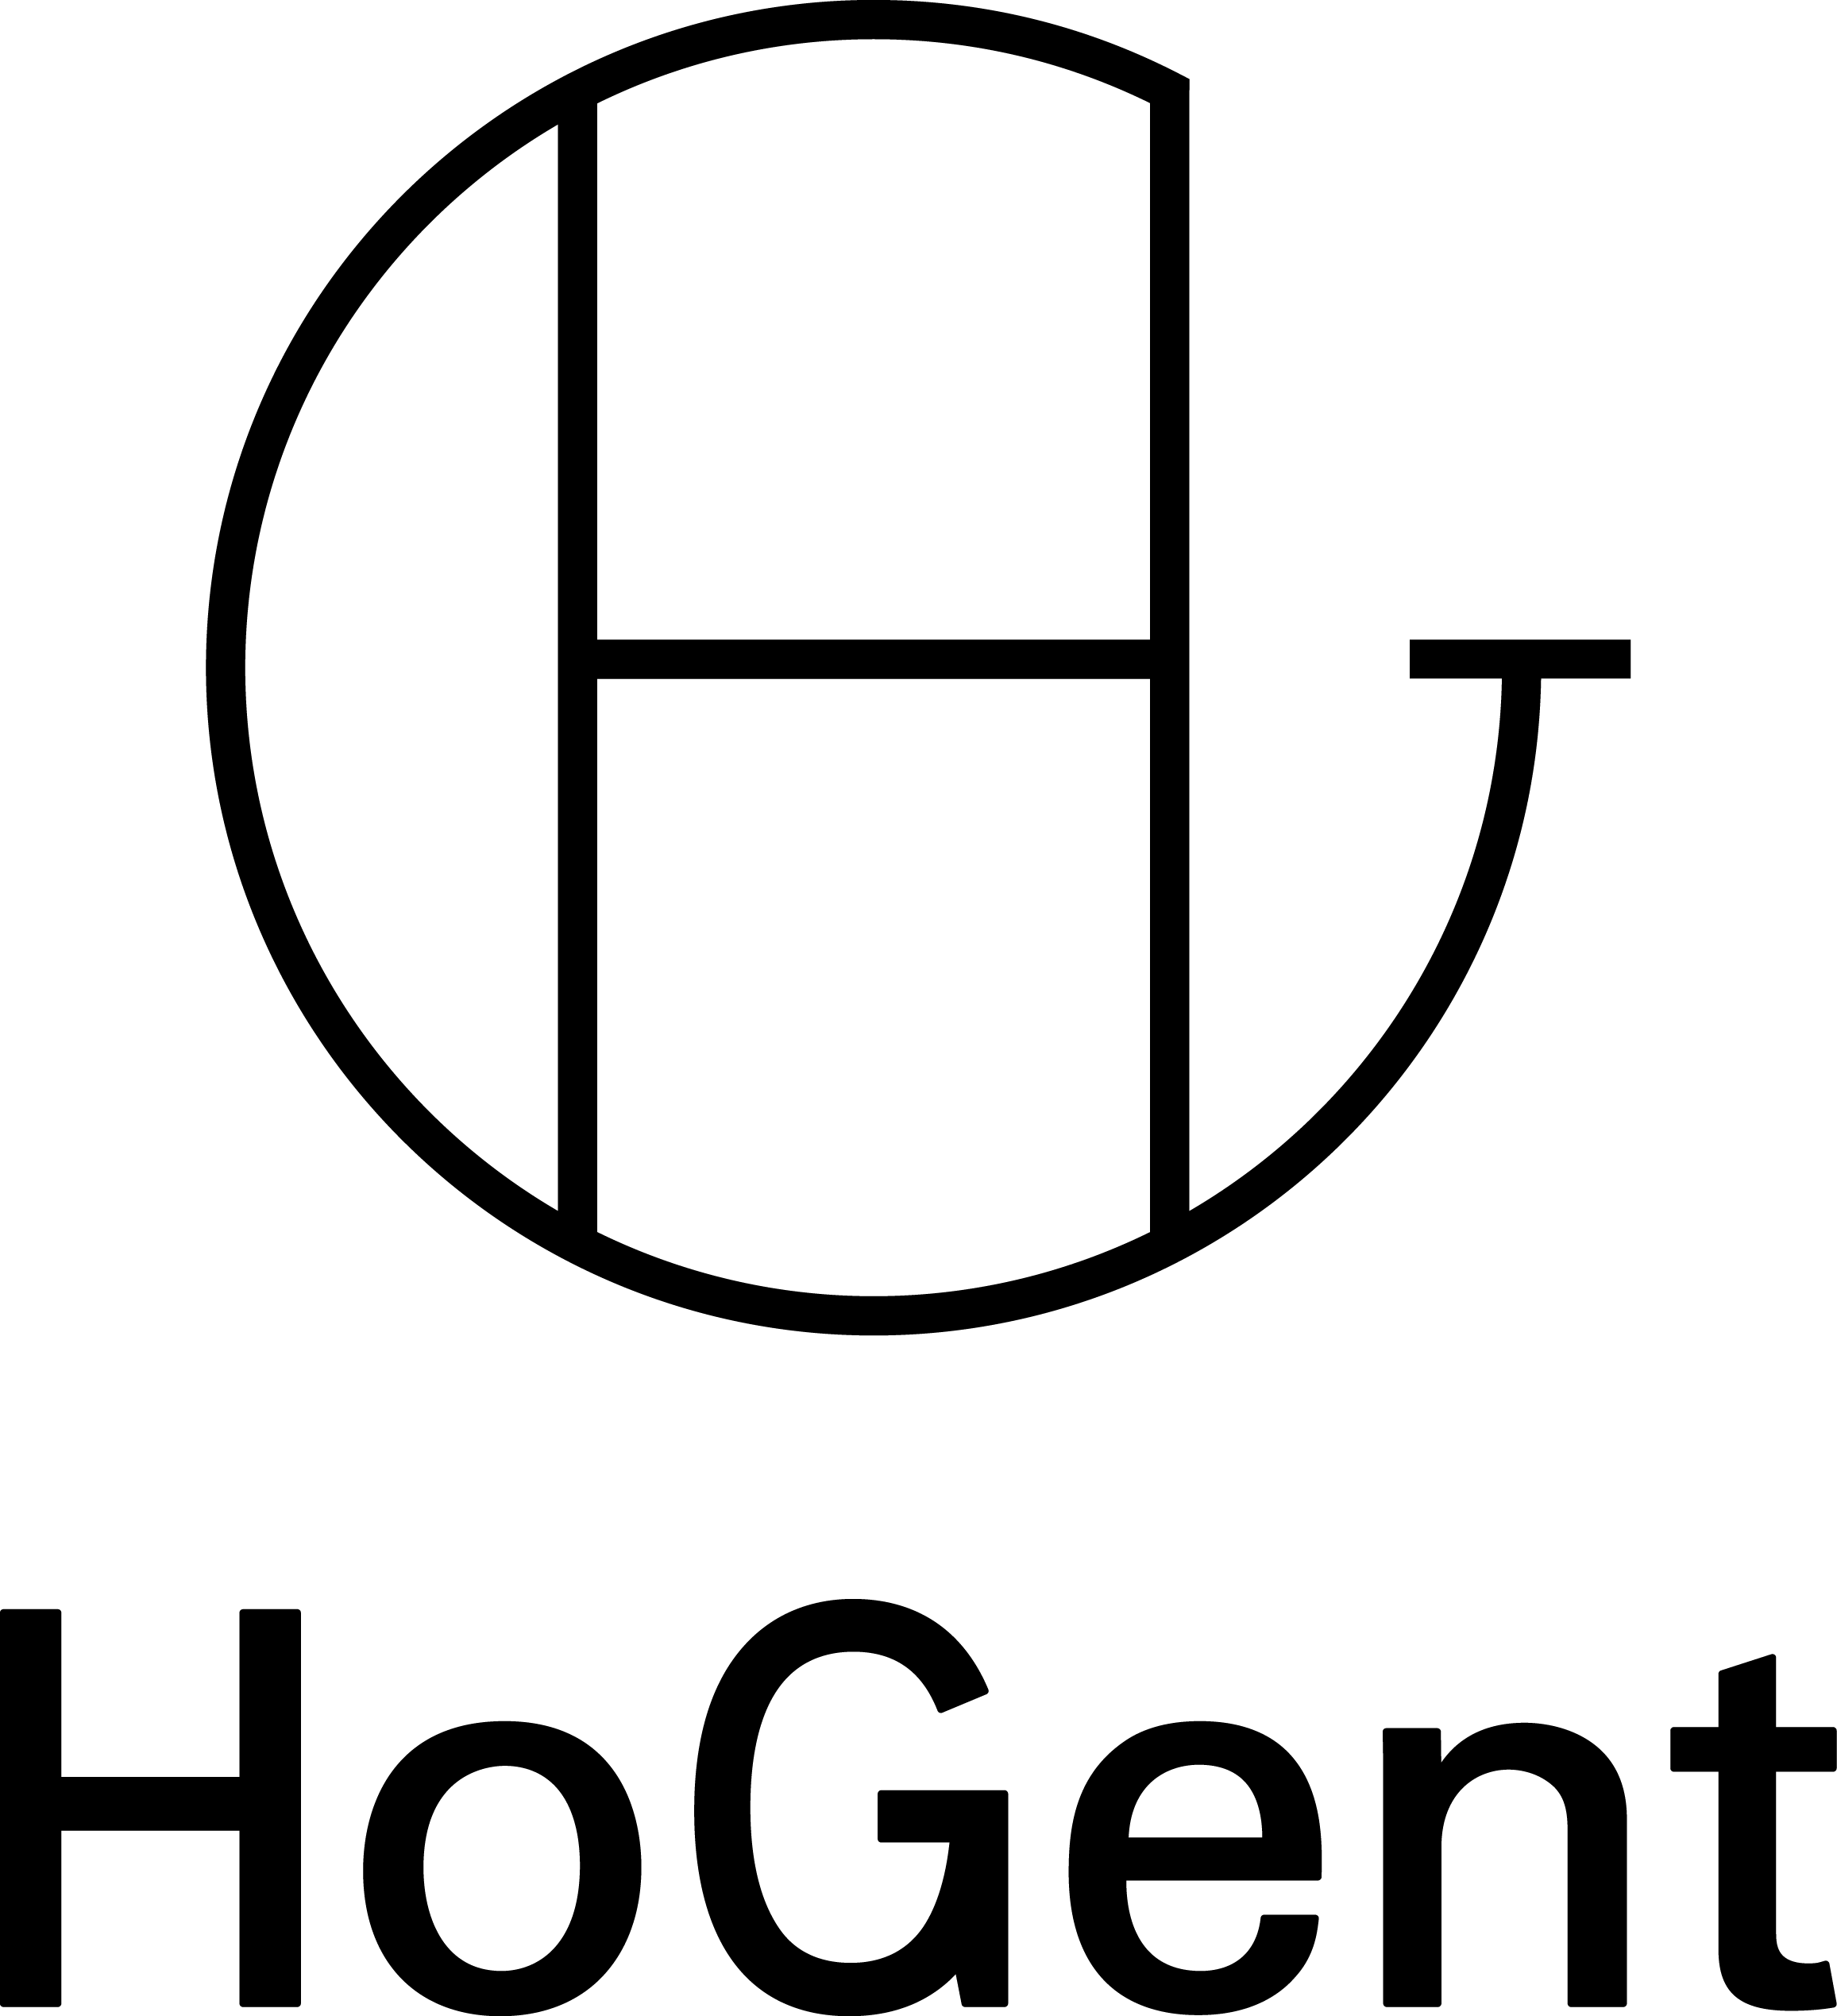
\includegraphics[width=2.5cm]{img/HG-beeldmerk-woordmerk}\\[.5cm]
    \faculteit\\[3cm]
    \titel
    \vfill
    \student\\[3.5cm]
    \rapporttype\\[2cm]
    Promotor:\\
    \promotor\\
    Co-promotor:\\
    \copromotor\\[2.5cm]
    Instelling: \instelling\\[.5cm]
    Academiejaar: \academiejaar\\[.5cm]
    \examenperiode
    \endgroup

  \end{center}
  \restoregeometry
\end{titlepage}

% Schutblad

\emptypage


\begin{titlepage}
  \newgeometry{top=5.35cm,bottom=1.5cm,left=1.5cm,right=1.5cm}
  \begin{center}

    \begingroup
    \rmfamily
    \faculty\\[3cm]
    \titleEN
    \vfill
    \student\\[3.5cm]
    \reporttype\\[2cm]
    Promoter:\\
    \promotor\\
    Co-promoter:\\
    \copromotor\\[2.5cm]
    Affiliation: \instelling\\[.5cm]
    Academic year: \academiejaar\\[.5cm]
    \examperiod
    \endgroup

  \end{center}
  \restoregeometry
\end{titlepage}


\begin{abstract}
% TODO: De "abstract" of samenvatting is een kernachtige (max 1 blz. voor een
% thesis) synthese van het document. In ons geval beschrijf je kort de
% probleemstelling en de context, de onderzoeksvragen, de aanpak en de
% resultaten.
\end{abstract}

\chapter*{Preface}
\label{ch:preface}

% TODO: Vergeet ook niet te bedanken wie je geholpen/gesteund/... heeft

\tableofcontents

% Als je een lijst van afkortingen of termen wil toevoegen, dan hoort die
% hier thuis. Gebruik bijvoorbeeld de ``glossaries'' package.

%%---------- Kern --------------------------------------------------------

\chapter{Introduction}
\label{ch:introduction}
\epigraph{``If you think that the internet has changed your life, think again. The IoT is about to change it all over again!''}{Brendan O'Brien}
The Internet of Things hasn't been around for a very long time, yet it's quickly becoming very popular and almost every tech company wants to be a part of it. It gained a lot of popularity around 2011 when IPV6 was released and it was around this time Gartner also took note of this trend and put it on their annual Hype Cycle for the first time. Around the same time of the growing popularity of the Internet of Things, the Bluetooth Special Interest Group released a new Bluetooth specification that was built for the Internet of Things: Bluetooth Low Energy. Gartner suggests that by 2020, around 20 billion `things' will be connected to the Internet of Things, a market that Bluetooth Low Energy wants to play a big role in. This thesis aims to provide an introduction to Bluetooth Low Energy and how one would go about connecting Bluetooth Low Energy to the Internet of Things. In this chapter the problem that the thesis is trying to find an answer for is elaborated, as well as the actual questions that need answering. An introduction about `AllThingsTalk' can also be found, a company that is trying to figure out how to connect Bluetooth Low Energy wearables with their Internet of Things infrastructure.

% De inleiding moet de lezer alle nodige informatie verschaffen om het onderwerp te begrijpen zonder nog externe werken te moeten raadplegen \citep{Pollefliet2011}. Dit is een doorlopende tekst die gebaseerd is op al wat je over het onderwerp gelezen hebt (literatuuronderzoek).

% Je verwijst bij elke bewering die je doet, vakterm die je introduceert, enz. naar je bronnen. In \LaTeX{} kan dat met het commando \texttt{$\backslash${cite\{\}}} of \texttt{$\backslash${citep\{\}}}. Als argument van het commando geef je de ``sleutel'' van een ``record'' in een bibliografische databank in het Bib\TeX{}-formaat (een tekstbestand). Als je expliciet naar de auteur verwijst in de zin, gebruik je \texttt{$\backslash${}cite\{\}}.
% Soms wil je de auteur niet expliciet vernoemen, dan gebruik je \texttt{$\backslash${}citep\{\}}. Hieronder een voorbeeld van elk.

% \cite{Knuth1998} schreef een van de standaardwerken over sorteer- en zoekalgoritmen. Experten zijn het erover eens dat cloud computing een interessante opportuniteit vormen, zowel voor gebruikers als voor dienstverleners op vlak van informatietechnologie~\citep{Creeger2009}.
\newpage{}
\section{Problem statement and research questions}
\label{sec:problemdefinition}
In this section, the goal is to quickly familiarize the reader with the subject this thesis is dealing about and which problems need to be solved in order to form a proper conclusion. First of all, the problem statement will be discussed where a quick sketch will be made as to why this thesis came to be. It will handle a subject that AllThingsTalk is very keen to discover for the development of their company and why combining Bluetooth Low Energy with their Internet of Things infrastructure is the next logical step for their business. Next, we'll look at the main question AllThingsTalk wants an answer for together with some smaller questions that logically follow it.

\subsection{Problem statement}
\label{subsec:problemstatement}
At the time of writing, there are already a lot of Bluetooth enabled products on the technology market. With the new Bluetooth Low Energy specification, Bluetooth is reaching out even further to products like socks\footnote{http://www.sensoriafitness.com/}, shoes\footnote{https://secure-nikeplus.nike.com/plus/products/basketball}, fitness bands\footnote{https://www.fitbit.com/} and more are being added to the list every day. The problem with these products is that in a lot of cases, the products only synchronize with a smartphone. Some manufacturers extend this connectivity by occasionally synchronizing the data the smartphone captures to their own proprietary cloud, where the data can be analyzed by both the company and the consumer. Most of the time, this is where the data cycle stops and it can't be further accessed by other parties, this is known as a closed loop system. In some cases, developers can still access the data with an API that communicates with the cloud service of the manufacturer, but this doesn't give any access to the raw sensor values and doesn't allow real-time data transfer.

On top of this, a lot of the devices being manufactured don't use standard SIG adopted BLE services, which makes interoperability with existing applications hard, if not impossible if authentication and encryption are added into the mix.

\subsection{Research questions}
\label{subsec:researchquestions}
There are a couple of questions that can be asked when combining Bluetooth Low Energy and the Internet of Things, and some of those questions alone could have multiple papers dedicated to them. For example, the matter of security will be a never ending debate, and even more concerns arise when talking about security in the Internet of Things. Another concern is privacy, but since this is very much a gray area, it's hard to formulate a one-sided conclusion on this matter. Some of these concerns will be addressed further in section \ref{sec:concerns}.

The main goals this thesis tries to fulfill are in essence very simple, but of course there are always some other questions that arise when looking at the big picture. These questions can be categorized as following, the questions in bold being the main research questions and the ones in plain text being auxiliary questions:
\begin{itemize}
	\item{\textbf{Can Bluetooth Low Energy wearables be used in an Internet of Things cloud infrastructure?}}
	\item{\textbf{Is is possible to use a smartphone as gateway to communicate with the AllThingsTalk cloud in real-time?}}
	\item{What is Bluetooth Low Energy?}
	\item{What is the difference between Bluetooth Low Energy and Bluetooth Classic?}
	\item{What are the pros and cons of this technology?}
	\item{What types of devices exist in Bluetooth Low Energy and how do they expose their data?}
\end{itemize}

\section{AllThingsTalk}
\label{sec:allthingstalk}
As you've probably already noticed, the company AllThingsTalk has been referenced a couple of times in the previous section. The reason for this is that this thesis is affiliated with the company and is being written for them. The company helped shape the vision of the thesis and offered some very interesting insights and ideas for subjects to write about, subjects which were very interesting for their own use.

AllThingsTalk was founded in July 2013 and their main objective is to `Make IoT ideas happen'. The company is already counting thirteen employees in two different countries, the headquarters being located in Ghent, Belgium. The office in Belgium counts seven people and is heavily focused on research \& development engineering, project management and sales \& marketing. The branch office is located in Belgrade, Serbia with the other six people, and their main focus is platform software development.

\subsection{History}
\label{subsec:atthistory}
AllThingsTalk has come a long way since the start of the company. They've received multiple Research \& Innovation grants from the government, the first being in September 2013 for building an open IoT platform: the AllThingsTalk Cloud. The second grant was received in May 2014, where the goal was to implement pattern recognition in their platform in order to help elderly people stay in their homes for a longer time. A third grant was acquired in February 2015, which was responsible for adding machine learning components to the platform.

Furthermore, they've hit some other major milestones throughout the years. In November 2014 they launched the first set of Rapid Development Kits for Internet of Things, where they added the Intel Rapid Development Kit in April 2015 and the LoRa Rapid Development Kit in November 2015. Other milestones include Internet of Things hackathons, the launch of IOTOPIA.be - a platform to introduce children in secondary schools to Internet of Things - and a LoRa partnership with Proximus, one of the largest telecommunications companies in Belgium.

\subsection{Products and services}
\label{subsec:attproductsservices}
The three main products and services AllThingsTalk offer are guidance, tools and cloud. 

For guidance, they offer IoT innovation workshops and private hackathons. This means that AllThingstalk organizes workshops for companies tailored to their needs, as well as hackathons which involve ideation, prototyping and more.

The second product is tools. AllThingsTalk offers a range of development kits that companies can purchase to accelerate their Internet of Things research. This includes kits like LoRa, Arduino Raspberry Pi, Intel Edison and Windows 10 IoT. `Hackathon in a Box' is also available, which helps companies to organize their own Internet of Things hackathon on their own.

Last but not least is the AllThingsTalk cloud, an Internet of Things prototyping platform which enables companies to connect their devices rapidly to the cloud, instead of hosting their own complicated infrastructure. Not only can this be used to prototype, but the platform is already being used in some very exciting projects like helping the elderly live in their home longer and an ongoing project which provides predictive maintenance in industries with machinery.

% TODO: Wees zo concreet mogelijk bij het formuleren van je
% onderzoeksvra(a)g(en). Een onderzoeksvraag is trouwens iets waar nog
% niemand op dit moment een antwoord heeft (voor zover je kan nagaan).

\chapter{Methodology}
\label{ch:methodology}
This chapter aims to explain what approaches and methods were used in the making of this thesis. It explains what methods were used for the two major parts of this thesis, being the research \& literature study and the Proof of Concept.

\section{Research and literature study}
\label{sec:researchlit}
Before starting the research, the most important question was `what does AllThingsTalk already know?'. Of course, being a company revolving around Internet of Things, it wouldn't be much use to dedicate a large section of this paper to it. However, some research had to be done about Internet of Things in order to understand some core concepts and technologies that are  used like transfer protocols such as MQTT and AMQP. A more abstract understanding was also needed, being how the Internet of Things works, what it's used for, why it's important and some more. This information is of course easily found online and wasn't of much use to include in this thesis.

That being said, the core subject of the research and literature study is about Bluetooth Low Energy. The research about this technology was done like you would research any other subject. Initially, the plan was to rely heavily on the official documentation of Bluetooth, but since the complete Bluetooth specification is over 2000 pages in length, a more practical approach was to purchase books that explain Bluetooth Low Energy, two of them being REFERENTIE BOEK 1 and REFERENTIE BOEK 2.

There are also training videos to be found on the Bluetooth website as well as various other short introductions to the technology all over the web, which provide a basic and quick understanding about the technology.

\section{Proof of Concept}
\label{sec:poc}
You don't get to know something without actually trying it out, which was one of the biggest focuses of the Proof of Concept. The actual goal of the Proof of Concept was more to provide the Bluetooth Low Energy layer than to connect to the Internet, as AllThingsTalk provides easy-to-use libraries in various language to connect to their platform.

In order to help speed up the learning process and quickly allow me to prototype and try out the technology, various devices were provided which offer a range of Bluetooth Low Energy profiles, services and characteristics, these terms are explained further in chapter \ref{ch:gatt}. These devices will shortly be introduced in chapter \ref{ch:android}.

The first goal of the Proof of Concept was to connect to a Bluetooth Low Energy device and read data on a smartphone. Various examples and repositories with source code provided some interesting insights as to how this API worked. Bluetooth also offers some starter kits to kickstart any project that wants to use Bluetooth Low Energy, including a very comprehensive and easy to use wrapper around the Android Bluetooth API.

Further goals of course include writing data and coupling the Bluetooth layer to the network layer, automatic service discovery and mapping, automatic generation of assets on the online platform and more. The most important concepts on how to do this are elaborated in chapter \ref{ch:android} and the accomplishments are listed in the conclusion, section \ref{sec:conclusion}.


% TODO: Hoe ben je te werk gegaan? Verdeel je onderzoek in grote fasen, en
% licht in elke fase toe welke stappen je gevolgd hebt. Verantwoord waarom je
% op deze manier te werk gegaan bent. Je moet kunnen aantonen dat je de best
% mogelijke manier toegepast hebt om een antwoord te vinden op de
% onderzoeksvraag.


%% TODO: de structuur en titel van deze hoofdstukken hangen af van je 
% eigen onderzoek. Elke fase in je onderzoek kan een eigen hoofdstuk krijgen. Kies telkens een gepaste titel. ``Corpus'' is *GEEN* gepaste titel
\chapter{Bluetooth Low Energy}
\label{ch:ble}
\epigraph{``Bluetooth Low Energy is going to change the way the world connects.''}{Robin Heydon}
Bluetooth has been around for a long time, and with the release of technologies like NFC it seemed like Bluetooth wasn't going to last for much longer. However, Bluetooth Low Energy has breathed new life into Bluetooth and it's now more popular than ever. Originally known as Wibree by Nokia, it was later merged into the Bluetooth standard after much consideration. This technology was built from the ground up to be as energy efficient as possible and will power the Internet of Things for years to come. Exciting updates are also on the way like mesh networking, allowing different nodes in a network to relay data to one another. In this chapter we'll be looking at what Bluetooth Low Energy actually is, what the key differences are between Bluetooth BR/EDR and Bluetooth Low Energy. Also worth investigating are the limitations of Bluetooth Low Energy and how this technology achieves low energy like no other.

\newpage{}

\section{What is Bluetooth Low Energy}
\label{sec:whatis}
In essence, Bluetooth Low Energy is the first open standard that consumes extremely low power. It has been built from scratch and has more things not in common than it does with Bluetooth, so the name can be a little bit confusing. Every component in this specification has been designed to consume as little power as possible, that's why this technology can also be called a `Coin cell' technology. This because a Bluetooth Low Energy enabled device can (theoretically, with normal usage) achieve battery life of around eight months on a coin cell battery. A great example of this are beacons, which can achieve a very long battery life if configured correctly. If fitted with a bigger battery, it can last for over two years. More information about the battery usage and how this low energy is achieved can be found in section \ref{sec:lowenergy}.

However, you might be thinking: if Bluetooth Low Energy is so great, why isn't it replacing other wireless technologies? The main reason for this is because it's very slow and has very little range. A couple of other limitations are present, but these will be more closely looked at in subsecion \ref{subsec:limitations}. Bluetooth Low Energy's main use is intended for Personal Area Networks, with a gateway in range that can relay data to a cloud service in order to connect various devices to the internet.

\section{Key differences between classic Bluetooth}
\label{sec:differencesclassic}
As the diligent reader probably already noticed, it seems that Bluetooth and Bluetooth Low Energy are worlds apart from one another. This is in fact very correct so it's hard to just list some differences and be done with it. In the next two subsections we'll look at why Bluetooth Low Energy is completely different from Bluetooth and should be seen as a new technology in its whole instead of an enhancement to the existing Bluetooth. The key limitations of the Bluetooth Low Energy specification are also addressed further in subsection \ref{subsec:limitations}.

\subsection{A new technology emerges}
\label{subsec:newtechnology}
A lot of authors are looking to compare Bluetooth with Bluetooth Low Energy, but this is an unfair comparison since the use cases for both of these technologies are completely different. As the name suggests, Bluetooth Low Energy is marketed for low energy devices like wearables and sensors, so it isn't here to replace other wireless technologies in the slightest where a continuous flow of data is required. They've also both been built around completely different core principles and have been designed to fulfill these requirements as best as possible.

\subsection{Limitations of Bluetooth Low Energy}
\label{subsec:limitations}
Bluetooth Low Energy doesn't bring all good news, but there are also a few key limitations to the technology, as with everything in life. Because the technology uses very little power, it's fairly easy to understand that the transmit power and transfer speeds aren't anywhere near other wireless technologies. In theory, Bluetooth Low Energy can achieve ranges of up to 65 meters and upcoming updates to the specification prove that this range will be increased even more. However, most manufacturers won't want their peripheral to transmit at such high range, because this will cause increased battery usage in turn. In practice, this range is of course much lower, as walls and even humans wreak havoc on the transmission of data.

Another limitation is the transfer speed. Again, in theory, Bluetooth Low Energy can have a (full packet) transfer speed of up to 1 Mbps\footnote{1 Mbps equals to 100 kilobytes per second.}. If you take into account the actual data contained in said packet and add up all of the overhead that goes into transferring a packet, 5 to 10 KB per second is a much more realistic representation. Knowing this, it's safe to assume that Bluetooth Low Energy won't be replacing WiFi any time soon.


\section{Bluetooth configurations}
\label{sec:bleconfigurations}
Bluetooth Low Energy is known by a variety of names on the market and while some of them are used to describe the same technology, in a few there's some differences to be found. `Bluetooth Low Energy' is mostly used as a catch-all name and can consist of a few different configurations. Some people assume `classic' or Bluetooth BR/EDR is also Bluetooth Low Energy, but this assumption couldn't be more wrong. If you have a product that specifies that you must have Bluetooth Version 4.0 or later, you're probably dealing with a Bluetooth Low Energy product.

Other names that can commonly be found are Bluetooth Smart (single-mode) and Bluetooth Smart Ready (dual-mode), these are both specifications of Bluetooth Low Energy but have one key difference between each other: backwards compatibility. Bluetooth Smart has been designed to only allow interoperability between itself and Bluetooth Smart Ready products. You'll usually see this configuration in wearable devices that connect to a smart phone, in this case the wearable is a Bluetooth Smart product and the smartphone is a Bluetooth Smart Ready product. Bluetooth Smart Ready on the other hand has been designed to allow communication with Bluetooth, Bluetooth Smart Ready and Bluetooth Smart products. Bluetooth Smart Ready is commonly present in the most recent smartphones, which will allow communication with Bluetooth products like headphones but also Bluetooth Smart products like a smart band. A more comprehensible and orderly overview of these technologies can be found in table \ref{table:configurations}.

\begin{table}[]
\centering
\caption{Compatibility table of Bluetooth specifications}
\label{table:configurations}
\begin{tabular}{|l|l|l|}
\hline
\textit{\textbf{Bluetooth version}} & \textit{\textbf{Supports BR/EDR}} & \textit{\textbf{Supports BLE}} \\ \hline
\textbf{Pre-v4.0}                   & v                                 & x                              \\ \hline
\textbf{4.x Bluetooth Smart}        & x                                 & v                              \\ \hline
\textbf{4.x Bluetooth Smart Ready}  & v                                 & v                              \\ \hline
\end{tabular}
\end{table}

\section{How low energy is achieved}
\label{sec:lowenergy}
There are a couple of techniques Bluetooth Low Energy uses to achieve low energy consumption. The fact alone that it can run off a 3 volt CR2032 coin cell battery and still retain 8 months of battery life proves that it is indeed a \textit{true} low energy technology. There are a couple of decisions that made it possible to achieve this low amount of energy consumption, some being the following:

\begin{itemize}
\item{\textbf{Use the radio as little as possible.} Keeping the radio on any wireless technology active requires quite a bit of power, which is also the case with Bluetooth Low Energy. By using the radio as little as possible, Bluetooth Low Energy can significantly increase its battery life. At a set interval, devices will broadcast advertising packets on the three advertising channels, which are explained more in chapter \ref{ch:gap}. After it advertises, it must listen briefly to any connection requests that follow it, in between these events the radio is simply turned off. The radio and the protocol stack, explained more in depth in chapter \ref{ch:protocolstack}, have also been designed to be as fast as possible. An advertising event, connection event, reading a single value of data and acknowledging the event can take as little as 3 milliseconds, which is vital in not only keeping the energy consumption to a minimum, but it also helps passively cool the radio.}

\item{\textbf{Keep packets very small.} Restricting the packet length to a maximum of 47 bytes allows very rapid packet transfers, which in turn contributes to keeping the radio off as much as possible. A maximum size packet of 47 bytes can be transferred in as little as 0.3 milliseconds. Keeping packets small also lowers the complexity of the transmitter and receiver, resulting in much lower power consumption than technologies that allow large packets.}
\end{itemize}

\chapter{The Bluetooth Low Energy protocol stack}
\label{ch:protocolstack}

\section{Controller}
\label{sec:stackController}

\subsection{Physical Layer}
\label{subsec:controllerPHY}

\subsection{Link Layer}
\label{subsec:controllerLL}

\subsection{Host Controller Interface}
\label{subsec:controllerHCI}

\section{Host}
\label{sec:stackHost}

\subsection{Host Controller Interface}
\label{subsec:hostHCI}

\subsection{Logical Link Control and Adaption Protocol}
\label{subsec:hostATTL2CAP}

\subsection{Attribute Protocol}
\label{subsec:hostATT}

\subsection{Security Manager Protocol}
\label{subsec:hostSMP}

\subsection{Generic Access Profile}
\label{subsec:hostGAP}

\subsection{Generic Attribute Profile}
\label{subsec:hostGATT}

\section{Application}
\label{sec:stackApplication}

\subsection{Application}
\label{subsec:applicationApp}

\chapter{Generic Access Profile}
\label{ch:gap}

\chapter{Generic Attribute Profile}
\label{ch:gatt}
\epigraph{``You can have data without information, but you cannot have information without data.''}{Daniel Keys Moran}
At the core of Bluetooth Low Energy communication, the Generic Attribute Profile or GATT is something a client will use in every data request or data push once a dedicated connection has been set up. It defines the way data is transferred in Bluetooth Low Energy and it uses the Attribute protocol, which is the protocol that stores Services, Characteristics, Descriptors and their respective values. In this chapter the general Attribute Profile and Protocol will be discussed, as well as the different data structures that come in to play. An example of an Attribute server will also be given using a standard SIG-approved Profile, as well as why and how one would implement their own Profile, either because the SIG-approved Profiles don't fit the use case or because the manufacturer wants to make the used technology more private.

\newpage{}

\section{Profiles}
\label{sec:profiles}

\section{Services}
\label{sec:services}

\section{Characteristics}
\label{sec:characteristics}

\section{Descriptors}
\label{sec:descriptors}

\chapter{Why Bluetooth Low Energy and Internet of Things}
\label{ch:BLEIOT}

\chapter{Android programming}
\label{ch:android}

\chapter{Discussion}
\label{ch:discussion}

\section{Conclusion}
\label{sec:conclusion}

\section{Concerns}
\label{sec:concerns}

A more concerning limitation is that Bluetooth Low Energy operates in the 2.4 GHz ISM frequency band, the same band that WiFi uses. They've chosen this band because the 2.4 GHz ISM band doesn't require any licensing cost, contributing to the very low chip cost of Bluetooth Low Energy devices. Luckily, Bluetooth Low Energy features an excellent algorithm to avoid major interference from WiFi, as it will avoid any channel that is being heavily used by other technologies.


\section{Future work}
\label{sec:futurework}

% TODO: Trek een duidelijke conclusie, in de vorm van een antwoord op de
% onderzoeksvra(a)g(en). Reflecteer kritisch over het resultaat. Zijn er
% zaken die nog niet duidelijk zijn? Heeft het ondezoek geleid tot nieuwe
% vragen die uitnodigen tot verder onderzoek?



\bibliographystyle{apa}
\bibliography{tin-bachproef}

%%---------- Back matter -------------------------------------------------

\listoffigures
\listoftables

\end{document}
